\pdfminorversion=4
\documentclass{beamer}

\usepackage[utf8x]{inputenc}
\usepackage[T1]{fontenc}
\usepackage{default}
\usepackage[portuges,brazil]{babel}
\usepackage{graphicx}
\usepackage{amsmath}
\usepackage{subfig}
\usetheme[compress]{Singapore}

\DeclareGraphicsExtensions{.jpg,.jpeg,.png}
\graphicspath{{../../imagens/}}

\begin{document}



% capa
\begin{frame}[plain]
  \begin{center}
    
\includegraphics[width=0.7in]{unicamp128}\\[0.5cm]
    \textsc{\large Universidade Estadual de Campinas}\\%[0.3cm]
    \textsc{\large Faculdade de Engenharia Mecânica}\\%[0.3cm]
    \textsc{\large ES952 - Trabalho de Graduação II}\\[1.0cm]


    \textsf{  \bfseries Desenvolvimento de um câmbio automático
  para bicicletas}

    \vfill
    % Author and project
    \begin{minipage}{0.4\textwidth}
    \begin{flushleft} \tiny
    \emph{Autor:}\\
    Paulo Silveira Machado \\
    RA: 024831
    \end{flushleft}
    \end{minipage}
    \begin{minipage}{0.4\textwidth}
    \begin{flushright} \tiny
    \emph{Orientador:} \\
    Prof. Dr. Luiz Otávio Saraiva Ferreira\\
    Faculdade de Engenharia Mecânica
    \end{flushright}
    \end{minipage}

  \end{center}

\end{frame}

% agenda
\begin{frame}[plain]
  \frametitle{Agenda}
  \tableofcontents
\end{frame}


% apresentação objetivos
\section{Apresentação}
\subsection{}
\begin{frame}
  \frametitle{Apresentação}
  \begin{itemize}
    \item Objetivo: Construir um protótipo funcional
    \item Premissas:
    \begin{enumerate}
      \item Baixo custo
      \item Adaptabilidade
      \item Configuração de parâmetros
      \item Interface com usuário
    \end{enumerate}

  \end{itemize}

\end{frame}


% justificativa
\section{Motivação}

\subsection{}
\begin{frame}
 \frametitle{Motivação}

  \begin{itemize}[<+->]
    \item Apelo ecológico da bicicleta
    \item Apelo à saúde
    \item Esporte de escolha (conhecimento de causa)
    \item Observações diárias
  \end{itemize}

\end{frame}

\section{Estudo}
% Problema físico
\subsection{}
\begin{frame}
  \frametitle{A transmissão ciclística}
  Destaque:
  \begin{itemize}
    \item \textit{Coasting}
    \item Mola de retorno
  \end{itemize}
\end{frame}

% bibliografia
\subsection{}
\begin{frame}
  \frametitle{Fontes de Estudo}
  \begin{itemize}%[<+->]
    \item Literatura Acadêmica
    \item Revistas especializadas
    \item Base de Patentes
      \begin{enumerate}
        \item EPO
        \item USPTO
      \end{enumerate}
  \end{itemize}
\end{frame}

\begin{frame}
  \frametitle{Fontes de Estudo}
  \begin{itemize}%[<+->]
    \item Literatura Acadêmica - Insatisfatória
    \item Revistas especializadas
    \item Base de Patentes
      \begin{enumerate}
        \item EPO
        \item USPTO
      \end{enumerate}
  \end{itemize}
\end{frame}

\begin{frame}
  \frametitle{Fontes de Estudo}
  \begin{itemize}%[<+->]
    \item Literatura Acadêmica
    \item Revistas especializadas - Pouca disponibilidade
    \item Base de Patentes
      \begin{enumerate}
        \item EPO
        \item USPTO
      \end{enumerate}
  \end{itemize}
\end{frame}

\begin{frame}
  \frametitle{Fontes de Estudo}
  \begin{itemize}%[<+->]
    \item Literatura Acadêmica
    \item Revistas especializadas
    \item Base de Patentes - Muita informação
      \begin{enumerate}
        \item EPO
        \item USPTO
      \end{enumerate}
  \end{itemize}
\end{frame}

\section{Desenvolvimento}
\subsection{}
\begin{frame}
  \frametitle{Bancada Experimental}
  \begin{itemize}
    \item Relativa facilidade na construção
    \item Para obter os sinais do sistema real
    \item Para atuar sobre sistema real*
  \end{itemize}
\end{frame}

\begin{frame}[plain]
 % fotos construção
 \begin{figure}
   \begin{center}
    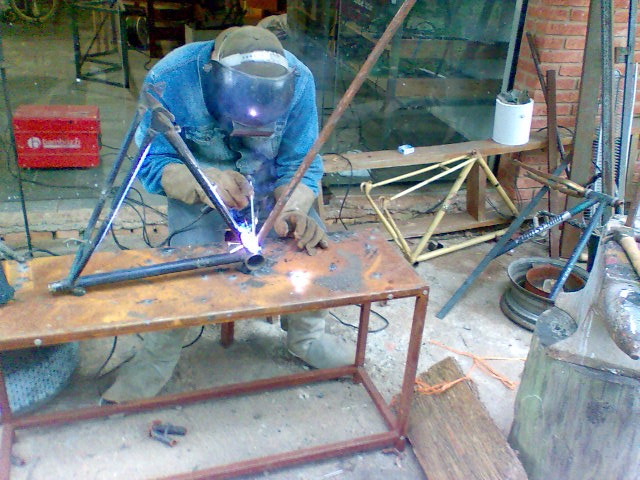
\includegraphics[width=3.5in]{making1}
  \end{center}
 \end{figure}
\end{frame}

\subsection{}
\begin{frame}
 \frametitle{Circuito de Controle}
  \begin{itemize}
    \item Microcontrolador
    \item Circuito de aquisição de sinais
    \item Montagem do atuador
  \end{itemize}
\end{frame}

\subsection{}
\begin{frame}
  \frametitle{Microcontrolador}
  \begin{itemize}
  \item Arduino Duemilenove (AtMega168):
    \begin{enumerate}
      \item PWM
      \item I/O Digitais/Analógicas
      \item 2 pinos de interrupção (\textit{falling/rising})
      \item Interface Serial
    \end{enumerate}
  \end{itemize}
\begin{figure}[h]
\begin{center}
 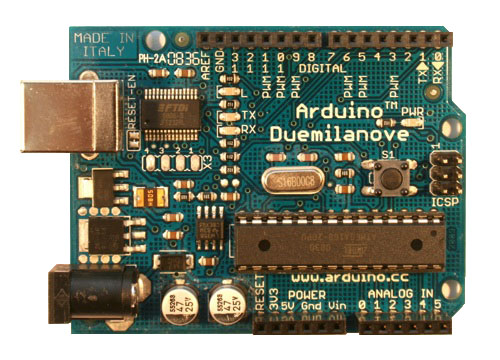
\includegraphics[width=2in]{duemilanove}
\end{center}
\end{figure}
\end{frame}

\subsection{}
\begin{frame}
  \frametitle{Aquisição de sinal}
  \begin{itemize}
    \item \textit{Reed Switchs}
    \begin{enumerate}
      \item Pró - Simples e barato
      \item Contra - \textit{Bouncing}
    \end{enumerate}
  \end{itemize}

\begin{figure}[h!]
 \centering
  \subfloat{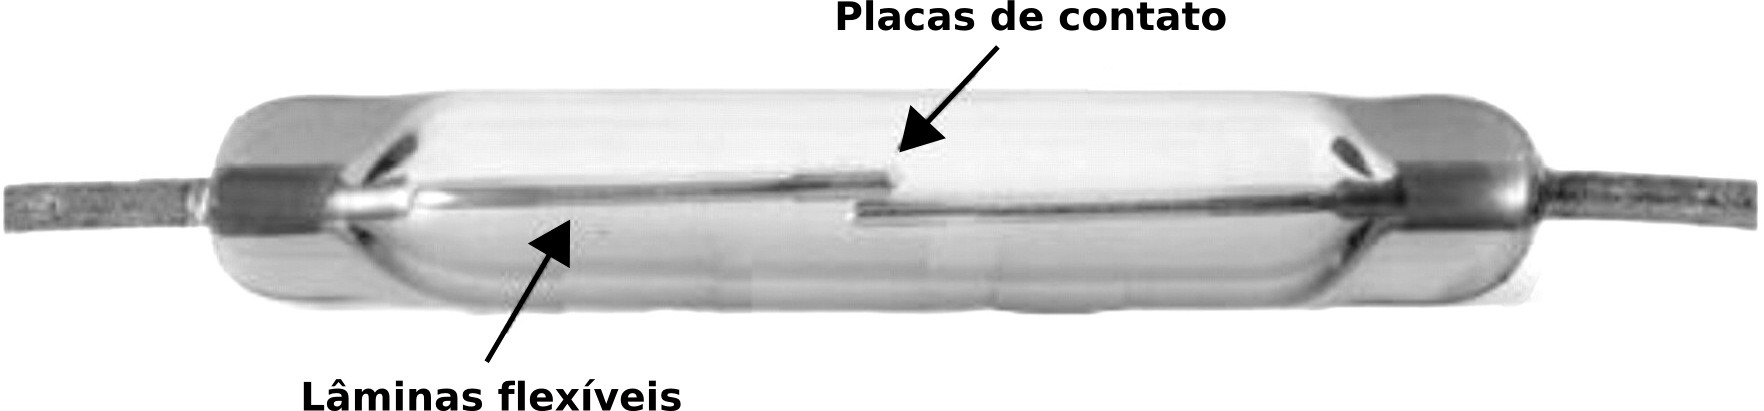
\includegraphics[width=1.5in]{reed}} \hfil
  \subfloat{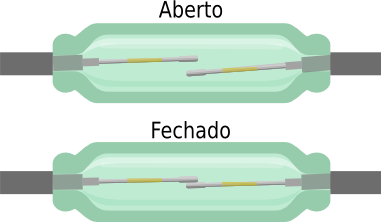
\includegraphics[width=1.5in]{reedschema}}
  \label{fig:reed}
\end{figure}
\end{frame}

\begin{frame}
 \frametitle{\textit{Debounce} em hardware}
  \begin{itemize}
    \item Filtro Passa-Baixa passivo RC
    \item Ruído de um \textit{reed} típico entre 1500-2000Hz
    \item Frequência máxima de ativação:
    \begin{equation}
  v = \omega r = 2\pi f r \Rightarrow v_{max} = 2\pi f_{max} r
\end{equation}
O diâmetro da roda com pneu foi medido em d=65cm = 0.65m. Para 90
km/h (25 m/s):
\begin{equation}
  f_{max} = \frac{\displaystyle v_{max}}{\displaystyle \pi d} =
\frac{\displaystyle 25}{\displaystyle \pi 0.65} = 12.243 Hz
\end{equation}

  \end{itemize}
\end{frame}

\begin{frame}
  \frametitle{Filtro RC passa-baixa, resistor \textit{pull-up}}
  \begin{center}
    \begin{figure}
        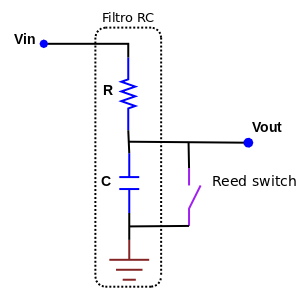
\includegraphics[width=2.8in]{lowpass}
    \end{figure}
  \end{center}
\end{frame}


\subsection{}
\begin{frame}
  \frametitle{Atuador}
  \begin{itemize}
   \item 
  \end{itemize}

\end{frame}

\subsection{}
\begin{frame}[plain]
\begin{figure}
 \centering
  \subfloat[Partes]{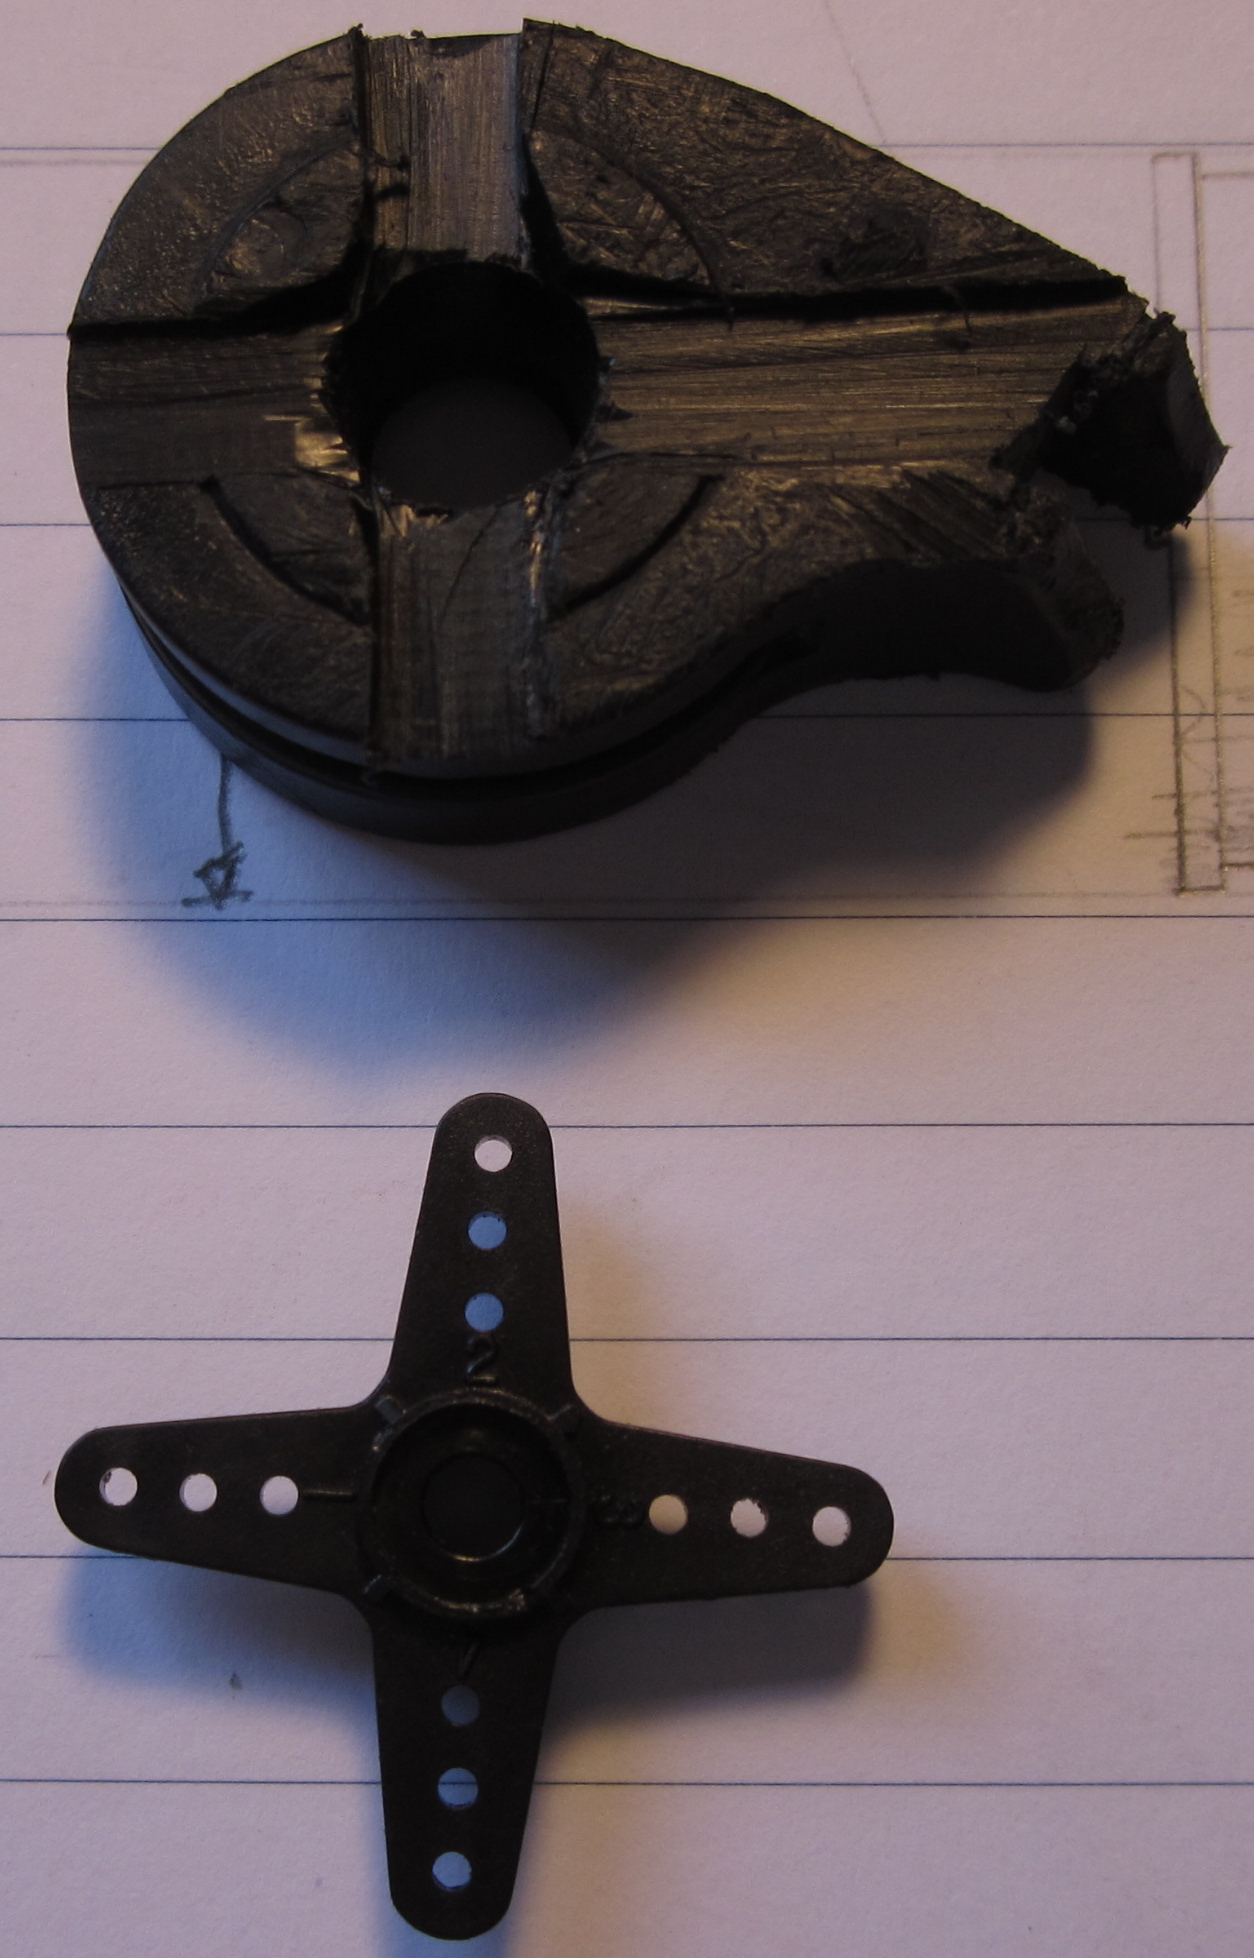
\includegraphics[width=1.3in]{polia1}} \hfil
  \subfloat[Partes Montadas]{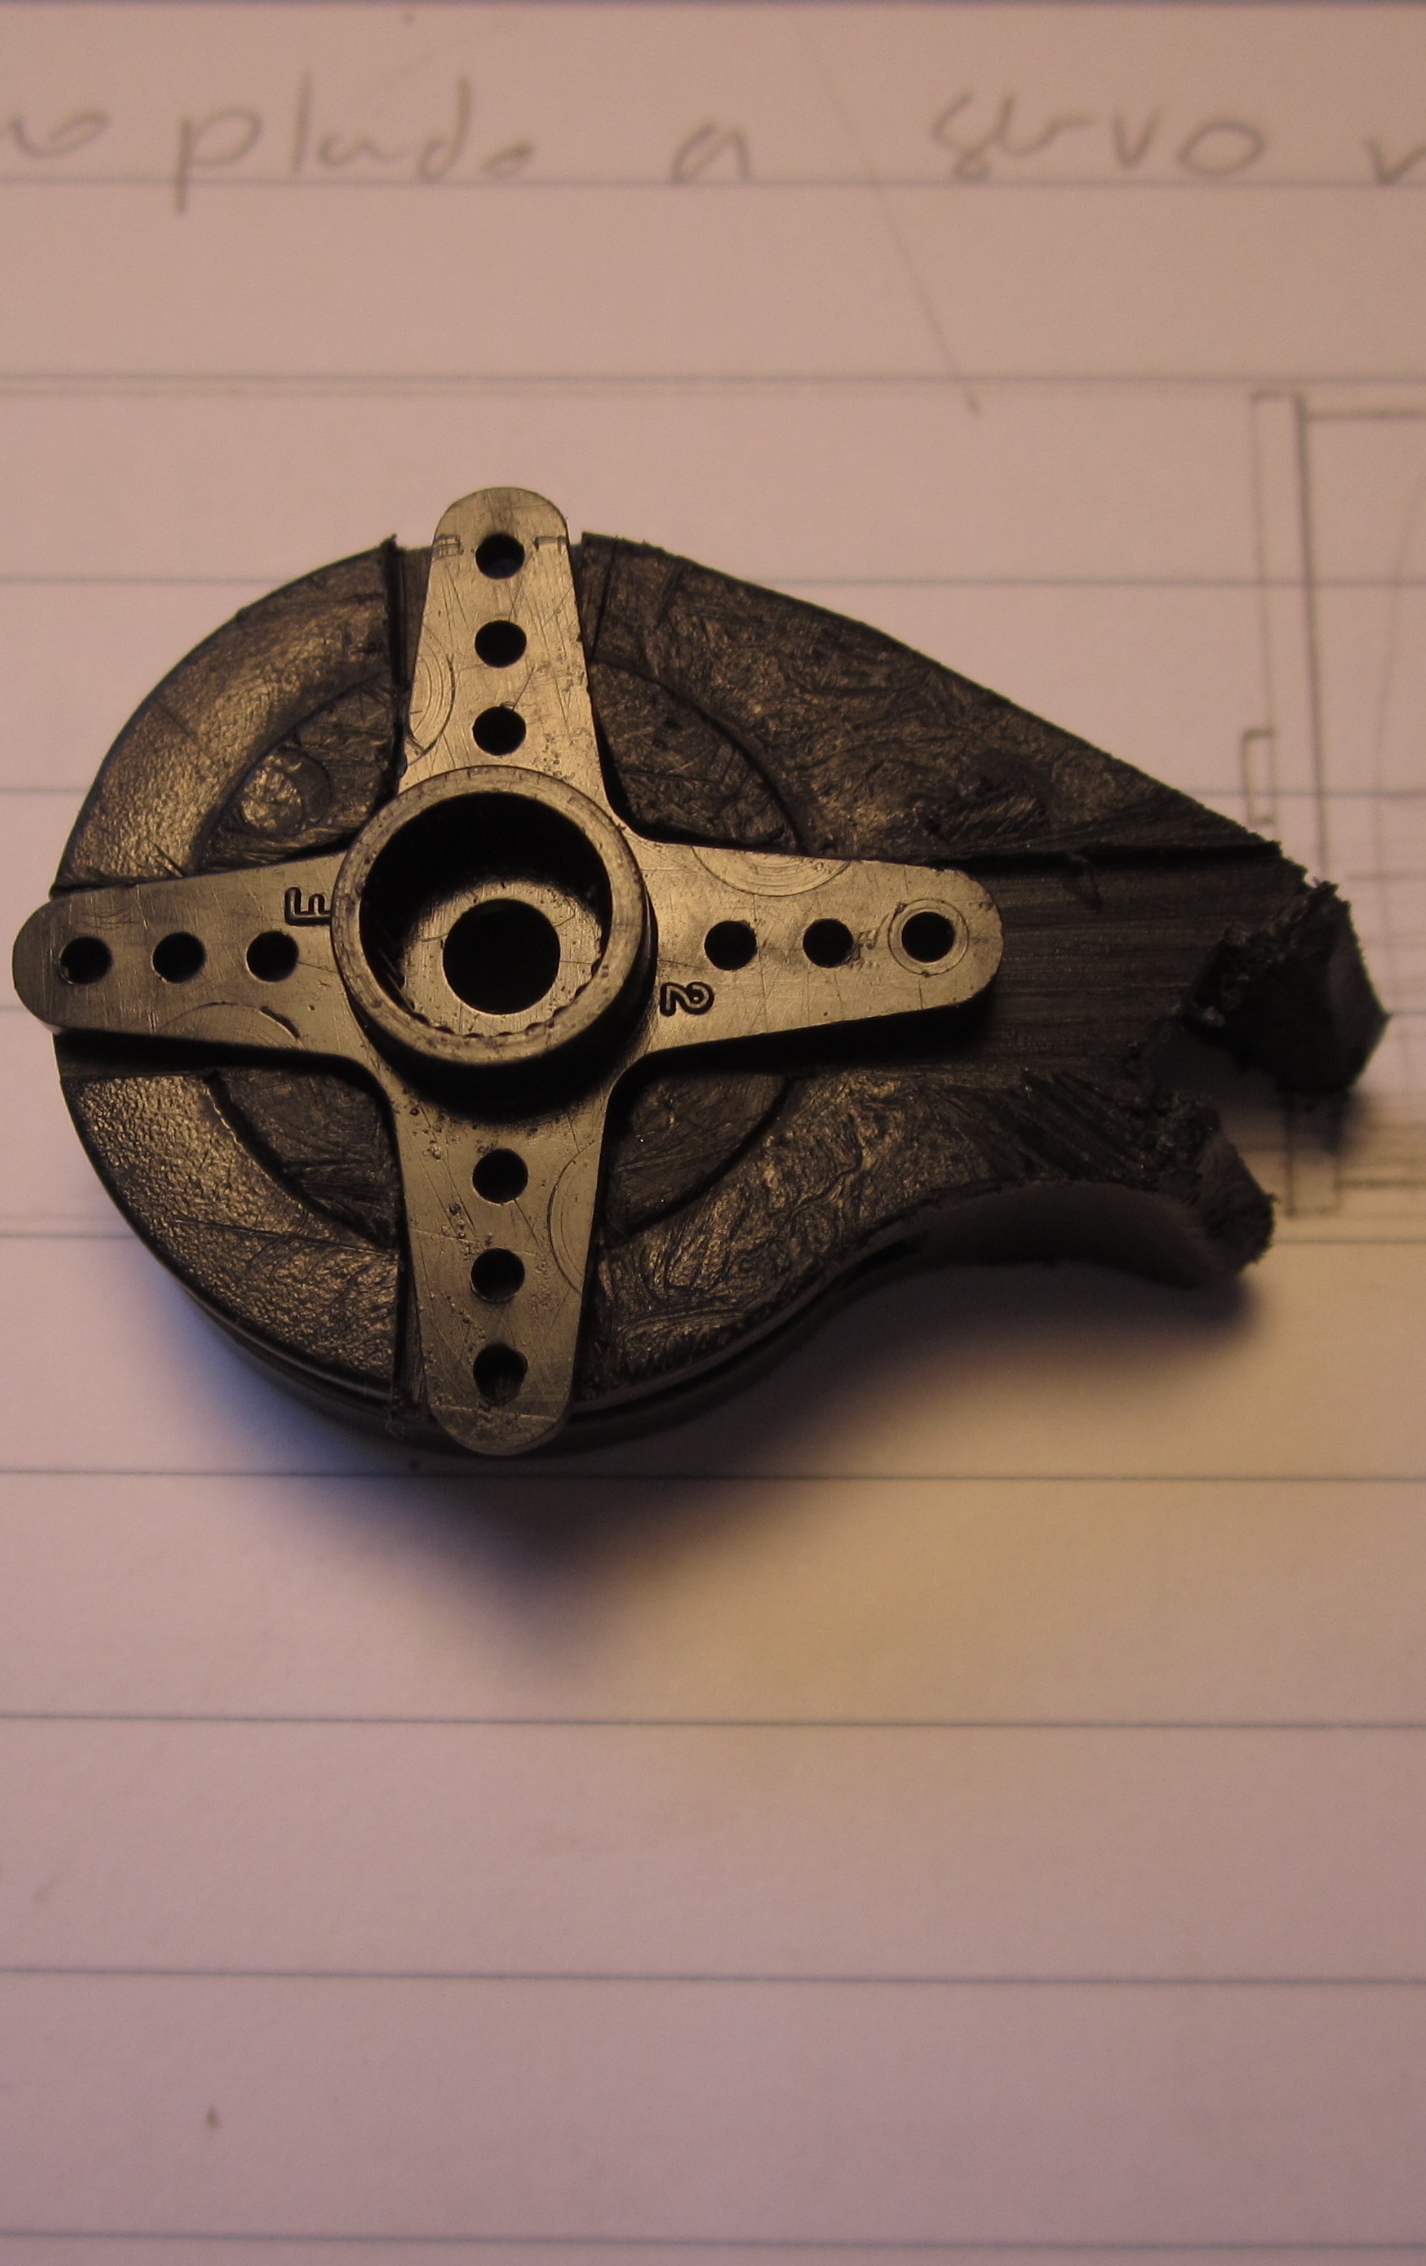
\includegraphics[width=1.285in]{polia2}} \hfil
  \subfloat[Atuador Completo]{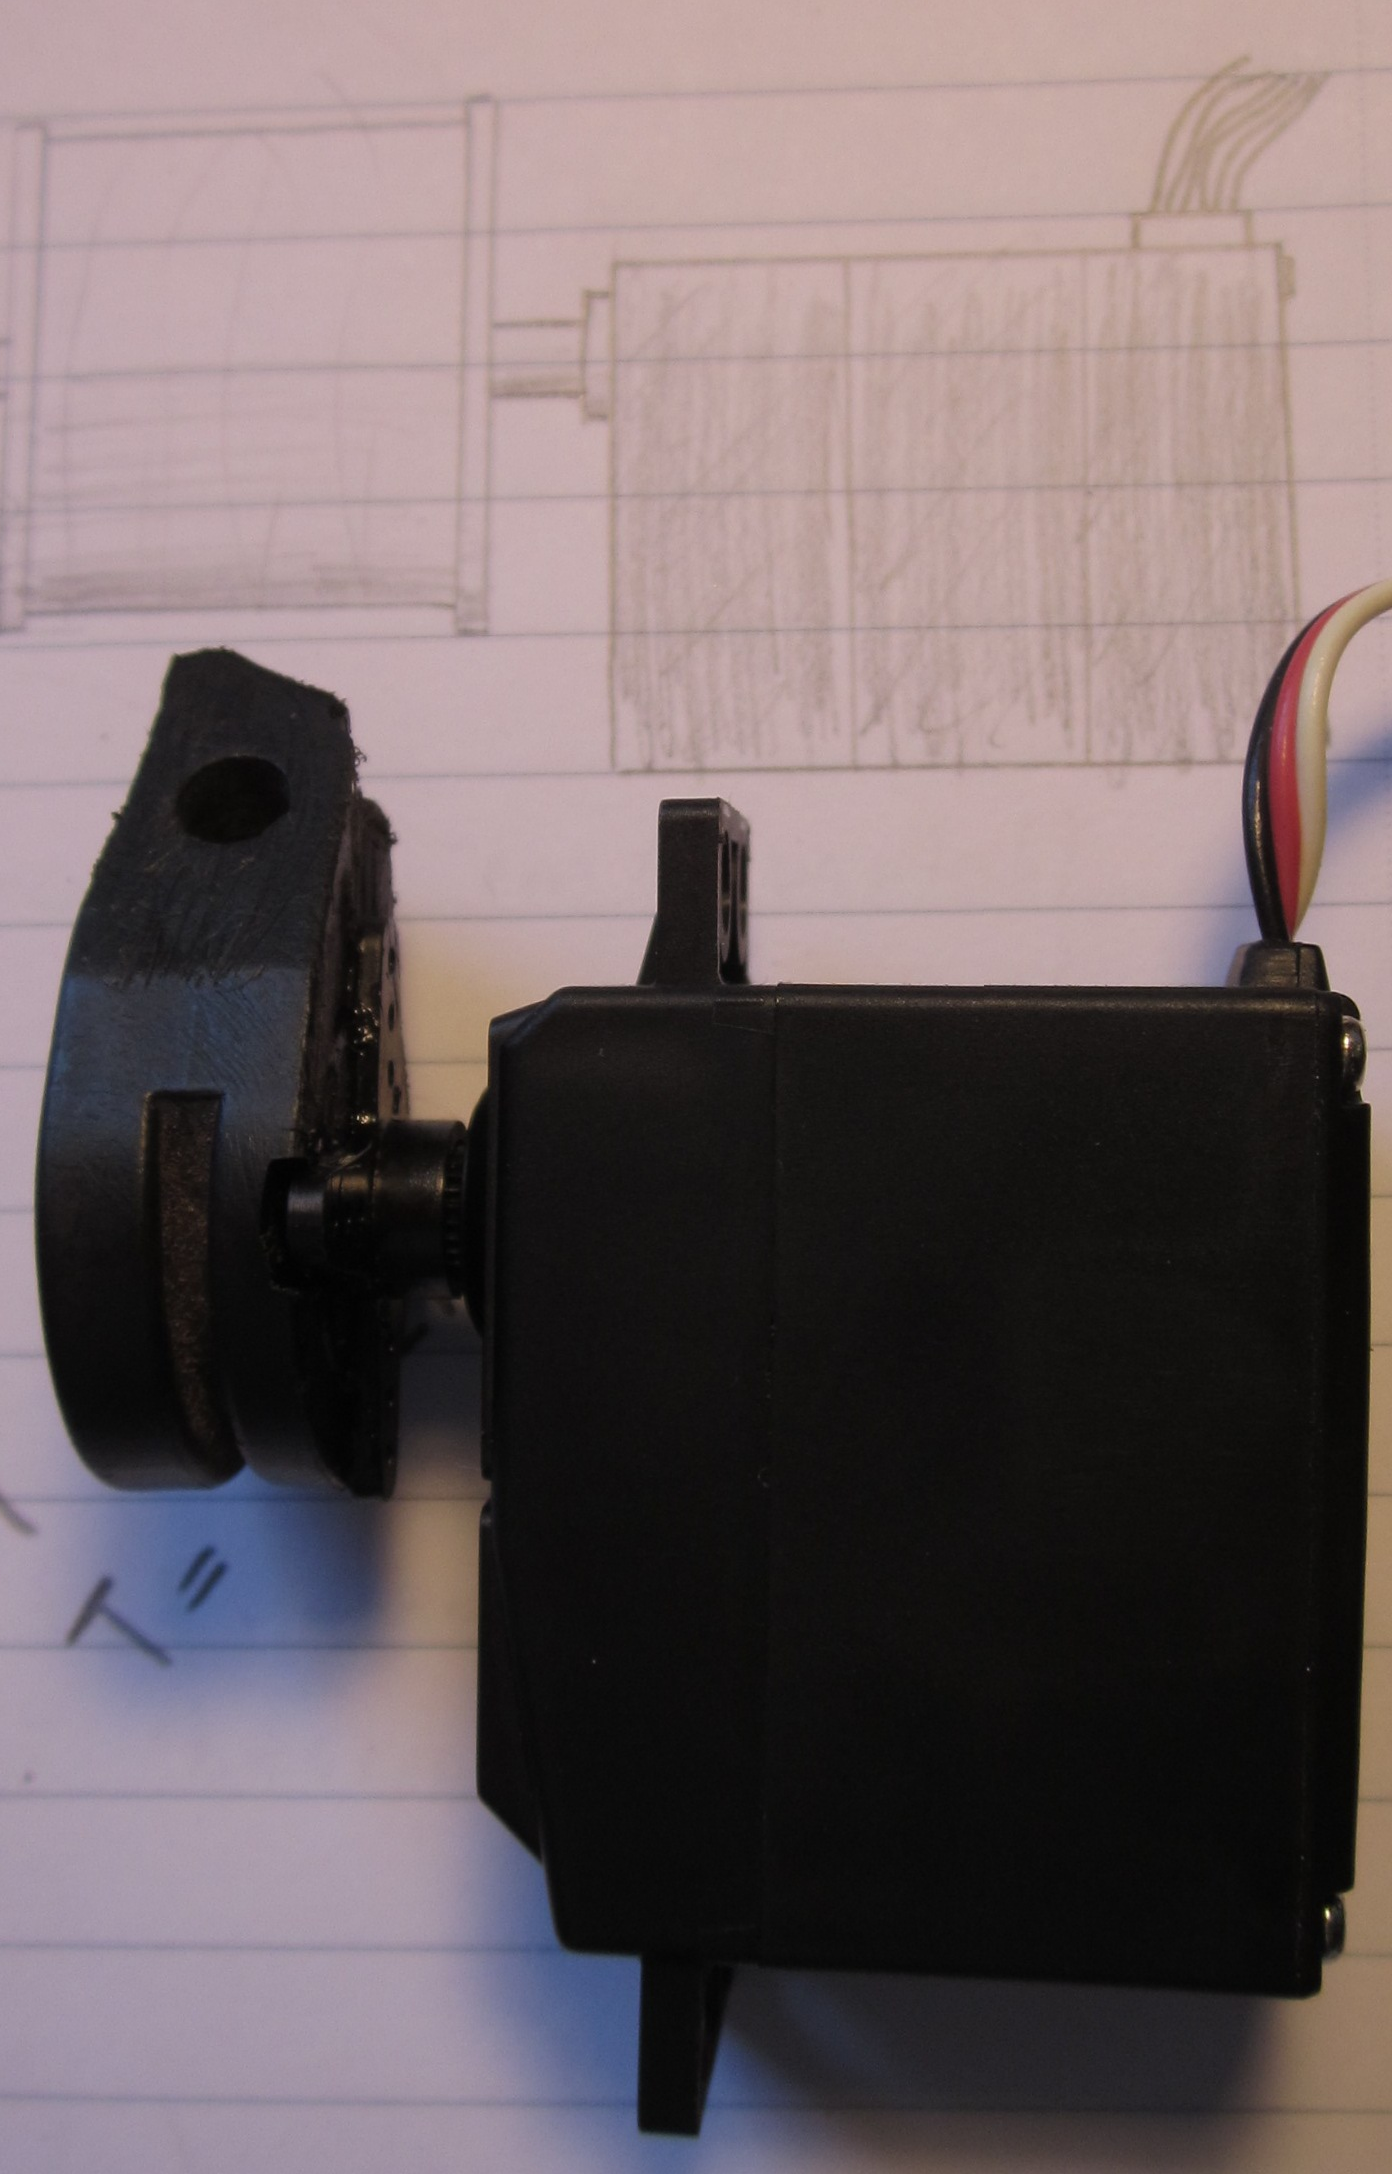
\includegraphics[width=1.3in]{polia3}}
\end{figure}
\end{frame}



\subsection{}
\begin{frame}
 \frametitle{Algoritmo de Controle}
\end{frame}

\section{Testes e Resultados}
\subsection{}
\begin{frame}
 \frametitle{Teste e Resultados}

  \begin{itemize}
   \item Montagem Completa
  \end{itemize}

\end{frame}

\section{Conclusão}
\subsection{}
\begin{frame}
 \frametitle{Conclusão}

  
\end{frame}

\subsection{}
\begin{frame}
 \frametitle{Perguntas?}
\end{frame}









\end{document}
